\subsection{Independent recovery assessment and failure boundary}
\label{sec:r23}
The frozen 385-tap FIR $ F $ and bypass receive the identical $ y=x+e $.
With the unchanged periodic recovery $ R $,
\begin{equation}
 z_0=y,\quad z_F=F(y),\qquad
 \widehat x_0=R(y),\quad \widehat x_F=R(F(y)).
 \label{eq:r23-branches}
\end{equation}
All 96000 reconstructed positions enter MSE/NMSE; no fitted gain, shift
or trimmed endpoint is allowed. Eq.~\eqref{eq:r23-metrics} gives units;
Eq.~\eqref{eq:r23-paired} gives paired reduction and error-SNR gain.
The mean gain averages individual logarithmic gains, not the logarithm
of mean MSEs. Error SNR includes deterministic distortion and differs
from target Gaussian SNR. The signal/error-power approach supports
this metric; correlation alone would
give one for $\widehat u=2u $ despite MSE $ P_u $.

Before drawing phase-1 noise I fix 50 complete records at each of
$-10,0,S_0,10,20,30,35,40 $ dB: 400 records, paths $(1,2,1,c,r)$.
The 35/40 dB diagnostics probe the predicted crossover without changing
the declared personal range. Whole records are independent; filtered
positions are not extra replicates. Mean intervals use the common
approximate t/CLT rule with $ R=50,m=1 $
(Appendix~\ref{app:statistics}; \citealp{scipy1153t,scipy1153sem}).
These pointwise mean intervals are neither simultaneous nor predictions
for a new record; count 50 makes no predeclared precision guarantee.

\begin{table}[!htbp]
 \centering
 \caption{Independent validation, 50 paired records per condition on all 96000 positions. Pointwise approximate 95 \% intervals describe mean gain; the dagger marks the personal baseline.}
 \label{tab:r23-quality}
 \footnotesize\setlength{\tabcolsep}{4pt}
 \begin{tabular}{rrrrr}
\toprule
Target $S$ & Mean MSE, no filter & Mean MSE, filter & Mean gain [95\% CI] & Wins \\
(dB) & (NPY units$^2$) & (NPY units$^2$) & (dB) & (/50) \\
\midrule
-10 & $7.2955\times10^{0}$ & $3.8900\times10^{-1}$ & 12.733 [12.703, 12.762] & 50 \\
0 & $7.3081\times10^{-1}$ & $3.8987\times10^{-2}$ & 12.730 [12.695, 12.766] & 50 \\
2.661$^\dagger$ & $3.9576\times10^{-1}$ & $2.1209\times10^{-2}$ & 12.711 [12.678, 12.743] & 50 \\
10 & $7.3101\times10^{-2}$ & $4.1467\times10^{-3}$ & 12.464 [12.431, 12.496] & 50 \\
20 & $7.3015\times10^{-3}$ & $6.1966\times10^{-4}$ & 10.714 [10.685, 10.743] & 50 \\
30 & $7.3097\times10^{-4}$ & $2.6878\times10^{-4}$ & 4.345 [4.329, 4.361] & 50 \\
35 & $2.3069\times10^{-4}$ & $2.4202\times10^{-4}$ & -0.208 [-0.219, -0.198] & 0 \\
40 & $7.2974\times10^{-5}$ & $2.3326\times10^{-4}$ & -5.047 [-5.055, -5.038] & 0 \\
\bottomrule
\end{tabular}

\end{table}


\begin{figure}[!htbp]
 \centering
 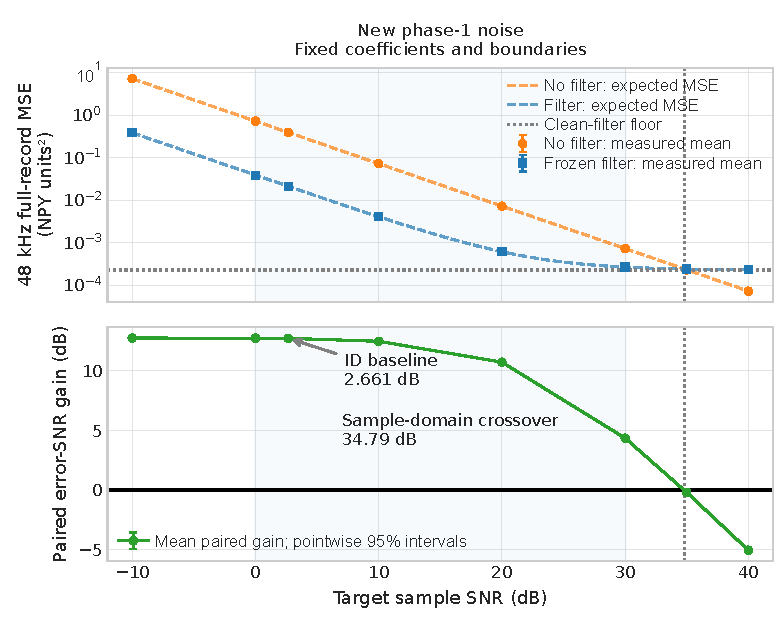
\includegraphics[width=.82\linewidth]{supporting/publication_r23_recovery_quality.pdf}
 \caption{Held-out mean MSE versus prediction (top) and paired gains with pointwise intervals (bottom). Shading: design range; line: prevalidation crossover.}
 \label{fig:r23-quality}
\end{figure}

\begin{samepage}
At the anchor point mean MSE falls from $\RtvPersonalBefore $ to
$\RtvPersonalAfter $ ($\RtvPersonalReduction $\%); mean paired gain is
$\RtvPersonalGain $ dB, interval $[\RtvPersonalLow,\RtvPersonalHigh]$.
All 50 improve at every tested level through 30 dB, including $-10 $ dB;
all 50 worsen at 35 and 40 dB. This is evidence at tested conditions,
not every realisation or every intermediate SNR. Fixed FIR distortion
persists after the input noise diminishes.
\end{samepage}

Prediction on the 48 kHz grid includes the old-Nyquist splitting correction
(Eq.~\eqref{eq:r23-reconstruction-energy}); sample-grid and recovered
powers are not silently equated. The no-filter gain is 0.999984375;
filtered gain $\RtvNoiseGainHigh $ and distortion $\RtvCleanHigh $ give
the plotted $ D_{48}+\sigma^2G_{48}$ prediction. At 40 dB, the first/last
768 positions, only 1.6 \% of duration, contribute
$\RtvHighEdgePercent $\% of filtered squared error. Edge shares use
aggregated sums, not averaged per-record ratios
(Eq.~\eqref{eq:r23-boundary-metrics}); they remain in every primary MSE.

Twelve checks cover inputs, freezing, disjoint seeds, grids and identities.
Twenty further audit checks use the separate cosine-series kernel
(Eq.~\eqref{eq:r23-audit-kernel}) and $K=64000$ real FFT to reproduce
372 scores/6696 design MSEs; the alternative-method replay in
Section~\ref{sec:r61} also checks all 400 validation inputs.
Records are in \path{metadata/r2_strict_checks.csv} and
\path{stage2/r23/results/}; these are replays, not extra data or retuning.
